% This is samplepaper.tex, a sample chapter demonstrating the
% LLNCS macro package for Springer Computer Science proceedings;
% Version 2.20 of 2017/10/04
%
\documentclass[runningheads]{llncs}
%
\usepackage{graphicx}
\usepackage{hyperref}
\usepackage{subcaption}
\usepackage{placeins}
\usepackage{float}
% Used for displaying a sample figure. If possible, figure files should
% be included in EPS format.
%
% If you use the hyperref package, please uncomment the following line
% to display URLs in blue roman font according to Springer's eBook style:
% \renewcommand\UrlFont{\color{blue}\rmfamily}

\begin{document}
%
\title{Asynchronous and Distributed Multi-agent Systems: an approach through actor model} %\thanks{Supported by organization x.}}
%
%\titlerunning{Abbreviated paper title}
% If the paper title is too long for the running head, you can set
% an abbreviated paper title here
%
\author{Felipe D. Reis\inst{1}\and
Tales B. Nascimento \inst{1}\and
Elizabeth F. Wanner\inst{1}\and \\
Carolina G. Marcelino\inst{2,3}\and
Henrique E. Borges\inst{1}}
%
\authorrunning{F. Reis et al.}
% First names are abbreviated in the running head.
% If there are more than two authors, 'et al.' is used.
%
\institute{Federal Center of Technological Education of Minas Gerais (CEFET-MG), Department of Computing, Brazil \\ \email{\{felipeduarte,henrique\}@lsi.cefetmg.br}\and
Federal University of Rio de Janeiro (UFRJ), Institute of Computing, Brazil \email{carolina@ic.ufrj.br}\and
University of Alcalá, Department of Signal Processing and Communication, Spain}
\maketitle              % typeset the header of the contribution
%
\begin{abstract}
	Agent-based and individual-based modeling have been widely used to simulate ecological systems. By and large, these simulations resort to classical concurrence mechanisms based on threads, shared memory and locks. Although these mechanisms seem to work fine for many multi-agent systems (MAS), notably those requiring synchronous communication between agents, they present severe restrictions in case of complex asynchronous MAS. In this work, we explore an alternative approach to handle concurrency in distributed asynchronous MAS: the actor model. An actor being a concurrent entity capable of sending, receiving and handling asynchronous messages, and creating new actors. Within this paradigm, there are no shared memory and, hence, no data race conditions. We introduce L2L (a short for: Learn to Live, Live to Learn) architecture, a biological inspired distributed non-deterministic MAS simulation framework, in which the autonomous agents (creatures) are endowed with a functional and minimal nervous system model enabling them to learn from its own experiences and interactions with the two-dimensional world, populated with creatures and nutrients. Both creatures and nutrients were encapsulated in actors. The system as a whole performs as a discrete non-deterministic dynamical system, as well as the creatures themselves. The scalability of this actor-based framework was evaluated showing the systems scales up and out $-$ many processes per processor node and in a computer cluster. A second experiment was realized in order to validate the architecture, consisting of an open-ended foraging simulation with both one or many creatures and hundreds of nutrients. Results from this specific actor-based version were compared to those from a classical concurrency version of the same architecture, showing they were equivalent, despite the fact that the former version scales a lot better. Moreover, results shown that exploration of the world was unbiased, leading us to conjecture that our system follows ergodic hypothesis. We argue that the actor-based model proves to be very promising to modeling of asynchronous complex MAS. 


\keywords{Distributed MAS \and complex agents \and situated cognition.}
\end{abstract}
%
%
%
\section{Introduction}
\label{sec:intro}
It is well known that simulating ecological systems in a individual-based (IB)  or an agent-based (AB) perspective, is more intuitive and faithful to reality instead of pure mathematical approaches \cite{Beecham1998}. Furthermore the complexity of those systems is naturally handled with AB models (ABM) \cite{An2012}.
Although the ABM is consolidated in literature, there is no general technique to handle the continued growth of complexity of multi-agent systems (MAS) \cite{An2012}. 

Despite the IB and AB modeling are not equivalent in concept, both have been used to understand the complexities of ecological management. Bousquet \& Le Page\cite{Bousquet2004} shows many concepts that bases ecosystems modeling and point the possibility of rich hierarchy simulation to understand natural phenomena from different perspectives. However, there is no mention concerning technological difficulties related to this kind of simulation.

In the field of cognitive science, the ABM has been used to  simulate and investigate the possibilities of various mind and brain theories. The LIDA architecture based on Global Workspace Theory \cite{Friedlander2008}. It specify for the agents a cycle of sensing, processing sensor signals and decision making that occur in parallel and asynchronously, while respecting the order of component stimulation to maintain the cognitive process coherence.

In the model MicroPsi - a multi-agent cognitive framework based on the Psy theory \cite{Bach2003} \cite{Bach2012} - the agent is composed of several components, including sensors and modulators which interacts with the environment, and a motivation set defined by the needs of the agent (\textit{i.e.},  energy, hunger, thirst). These needs trigger the internal cognitive process of the agent and modulate its behavior. There is also a component that coordinate the allocation of the resources to internal components during execution. 

Modeling natural phenomena has to take in account the simultaneity of various events. In real cases the agent and the environment interacts each other through a stimulation process simultaneously \cite{Maturana1987}. From this perspective, the actor model is a powerful technique to design this kind of interaction. In the actor model, "computation  is  conceived  as  distributed  in space where computational devices communicate asynchronously and the entire  computation  is  not  in  any  well-defined  state" \cite{Hewitt2012}. Following this definition, actor model helps to design and implement systems which it events  shall happen asynchronously and simultaneously. Furthermore, as the computation is defined as distributed, this approach gives the model the ability to scale over many machines, without changing fundamental implementation decision. 

The architecture proposed in this article called L2L (Live to learn, learn to live), a biologically inspired MAS architecture, is a new implementation of a former version previouly described by \cite{Campos}. This former version could only be ran in one machine with a narrow limit on the number of agents, thus preventing ecosystems simulations. The current implementation specify each creature and nutrients as actors, which interact through message passing. The results shows a remarkable enhancement in system scalability, allowing further simulations involving hundreds of complex creatures in a computer cluster. 

The organization of this article follows: the L2L architecture is presented together with the actor model in \autoref{sec:model}; experimental results are discussed in \autoref{sec:results}, then follows the conclusion.

\section{Proposed Model}
\label{sec:model}

\subsection{L2L architecture}
\label{subsec:l2l}
L2L is a biologically inspired architecture of embodied and embedded cognition that has been used to study foraging and action selection \cite{Campos}. The architecture consists of a two-dimensional surface of a toroidal world, which is populated by artificial creatures (active components) and nutrients (passive components). Both of them interact asynchronously exchanging stimuli. The nutrients have different nourishing values and the creature has no a priori knowledge about those values neither the food distribution around the world. 

The creature is endowed with a basic nervous, emotional and sensory-motor systems, and various internal ``organs'' that interacts asynchronously with each other. This interaction represents the biological nervous and hormonal stimulation and is implemented via threads and shared memory. The access to shared memory is controlled by locks, and is implemented by all threads.

The creature internal state is modulated, but not determined, by the external stimuli received through the sensory system. The whole system operates in a non-deterministic dynamics through time and space. It is expected that the behaviour of adaption, and thus establishment of food preferences, emerge from the inner emotional-cognitive process. However, is not the focus of this paper describe that process, for more details see \cite{Campos}.

The intrinsic model's complexity combined with implementations decision about concurrency (use of shared memory, threads and locks) made a single creature computationally heavy, limited to two creatures by computer core. Increasing this number causes the creature behavior becoming incoherent in sense that, behavioral dynamics loose congruence with inner nervous system dynamics. This upper bound was severely limiting to studies involving ecological simulations, e.g. socio-genesis, semiotics, population dynamics, etc. Aiming to use more machines to run a large number of creatures in one simulation, it is necessary to decouple them from the shared memory. The choose alternative to achieve this goal relies on the actor model.

\subsection{The Actor Model}
\label{subsec:actors}
An actor is a mathematical concept of a universal primitive of digital computation\cite{Hewitt2012}. The actor is an entity capable of sending messages, receiving and handling messages, as well as creating new actors. The actor model is by conception concurrent, and all the communications are asynchronously done through exchange, \textit{i.e.},  there are no shared memory and hence no data race conditions. The messages in the actor model are decoupled from the sender and delivered by the system on a best efforts basis\cite{Hewitt2014}. There are no guarantees as to the ordering of messages, so, the system must be carefully prepared to handle the incoming messages no matter their order.

%% Discutir outros modelos de atores implementados: os de erlang e o quasar
There are many implementations of the actor model, \textit{e.g.}, Erlang - a programming language which its concurrency mechanism works  asynchronously as actors \cite{Armstrong2007}, and Quasar\footnote[1]{http://docs.paralleluniverse.co/quasar/} library that runs over Java Virtual Machine (JVM). The Akka toolkit\footnote[2]{http://akka.io/} is one of these, and we choose it because it best fit the technologies we already used. It does not respects all of the theoretical description from above because of technological constraints and practical factors. Since Akka runs on a JVM and is a library, it cannot strictly guarantee data separation from the actors. Also, the toolkit implements message ordering between pairs of actors. All actions taken by an Akka actor are in response to some received message, whether sent by itself or by another actor, i.e the system is reactive. Yet, it does not guarantee message delivery between two computers.

The advantage of using the actor model is that it provides a higher level of abstraction when compared with the classical concurrent model. Due to the fact that there are no data race conditions, the model scales up, using efficiently the available resources in one machine. Also, the toolkit we used provides an implementation that works with multiple machines, enabling scaling out. In the new implementation, the actor model is used to simulate a two-dimensional world which is composed of artificial creatures and nutrients. Either creatures and components are encapsulated in actors and they exchange stimuli with each other. There is an underling control structure responsible for managing the simulations and replenish the nutrients, if necessary. This structure is shown in the Fig \ref{diagramaAtores}. 

As said previously the creature is an actor, and it encapsulates its nervous systems and its other subsystems. Those creature components still use threads as the concurrence model and must run in the same machine. In order to manage those creatures, there is a holder actor that create and keep track of them, and a repository actor that delegate which holder will receive the next creation order. The nutrient repository and holder are analogous to its creature counterparts. The simulation manager is an actor responsible to create, start and stop a given simulation, \textit{i.e.}, given how many creatures and nutrients are populating the world, it asks the repositories to create them and wait for the ready response. When everything is configured it send messages to start the simulation.

For the control messages (those exchanged by control actors), we implemented a synchronous protocol. It increases the reliability of message delivery with a penalty on the overall performance. A miscommunication between this kind of actors would result in simulation failure. Since this kind of communication is not prevailing, the performance cost is acceptable. The creature and nutrient actors communicate with the collision detector actor using a fire-forget (best effort) method, that is faster than the synchronous method. Since these actors produce the statistics for the simulation, some message loss is tolerable.


\begin{figure*}
	\centering
	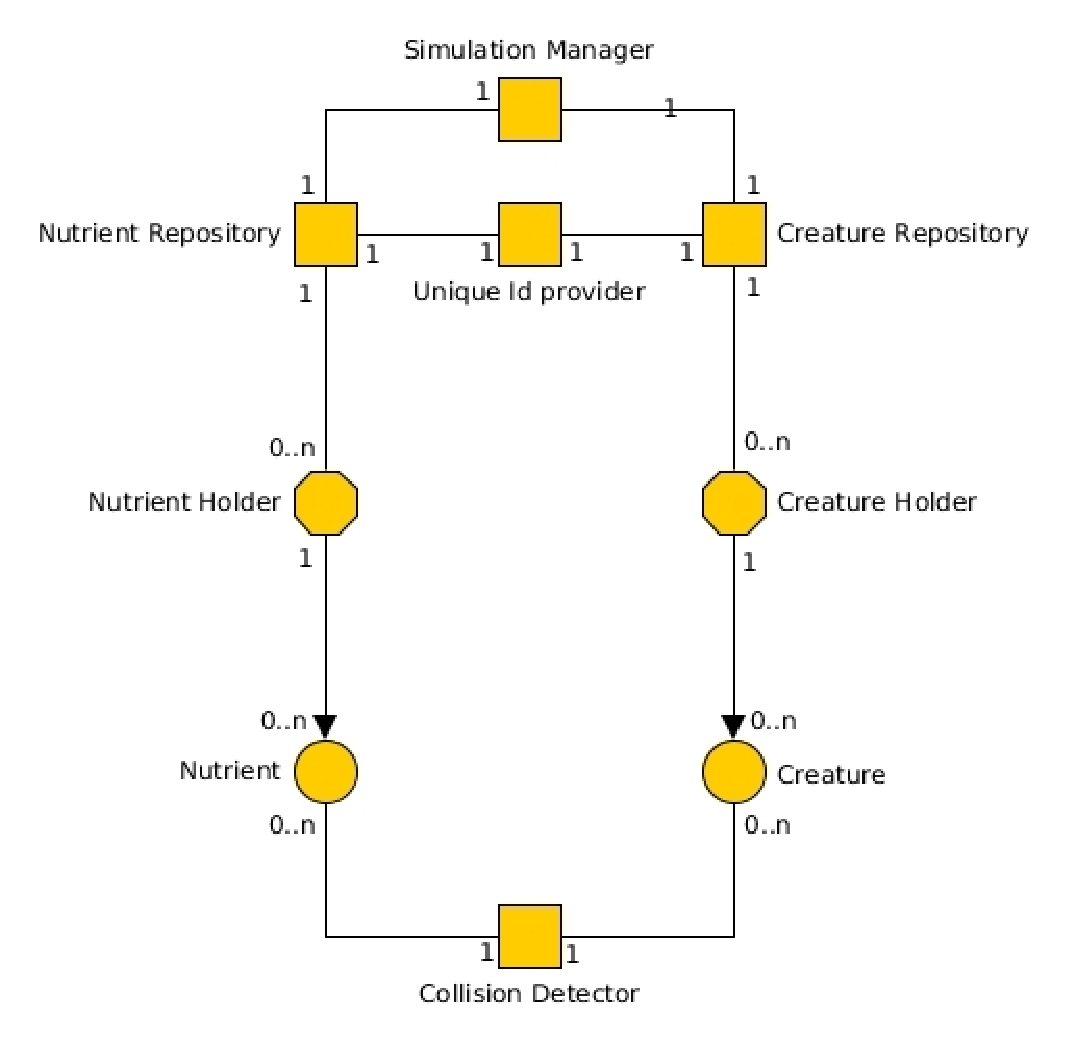
\includegraphics[width=14cm]{images/diagramaAtores}
	\caption{Block diagram for the implemented model. All but the Creature and Nutrient are control actors. Each simulation must have at least one of each type of actor, and at most one each actor represented by a square. The communication between the Creature and Nutrient actors with the Collision detector are fire-forget. The other communications have a acknowledge mechanism}
	\label{diagramaAtores}
\end{figure*}

\section{Experimental Results}
\label{sec:results}

We propose two experiments to validate the present model and evaluate its scalability. They were performed in a small computer cluster, composed of eight slave machines and a master connect through a Gigabit Ethernet network. The cluster machines has 3 Intel i5-3470 processors, 32 GB dual channel DDR3 RAM. In those simulations a number of artificial creatures were created, without any kind of \textit{a priori} knowledge about the world, in a virtual world filled with different kind of nutrients. In both experiments the nutrient density was maintained constant during the executions, \textit{i.e.},  if a nutrient is eaten, another one of the same type is promptly created in an aleatory position (uniform distribution). 

\subsection{Model scalability}

In order to evaluate the scalability of the implementation using the actor model, we measured the number of averaged exchanged external stimuli between actors as a function of computer nodes running, while keeping the ratio of creatures per machine constant. We start with 10 creatures and 90 nutrients, using one machine for the creatures and another one for the rest of the system. A simulation comprises 30 runs for each configuration, and each run was interrupted after 300 seconds, as our purpose was to evaluate only system scalability. It is worth noticing, however, that L2L is designed for open-ended simulations (see  Fig. \ref{inferno}). 

\begin{figure}
	\centering
	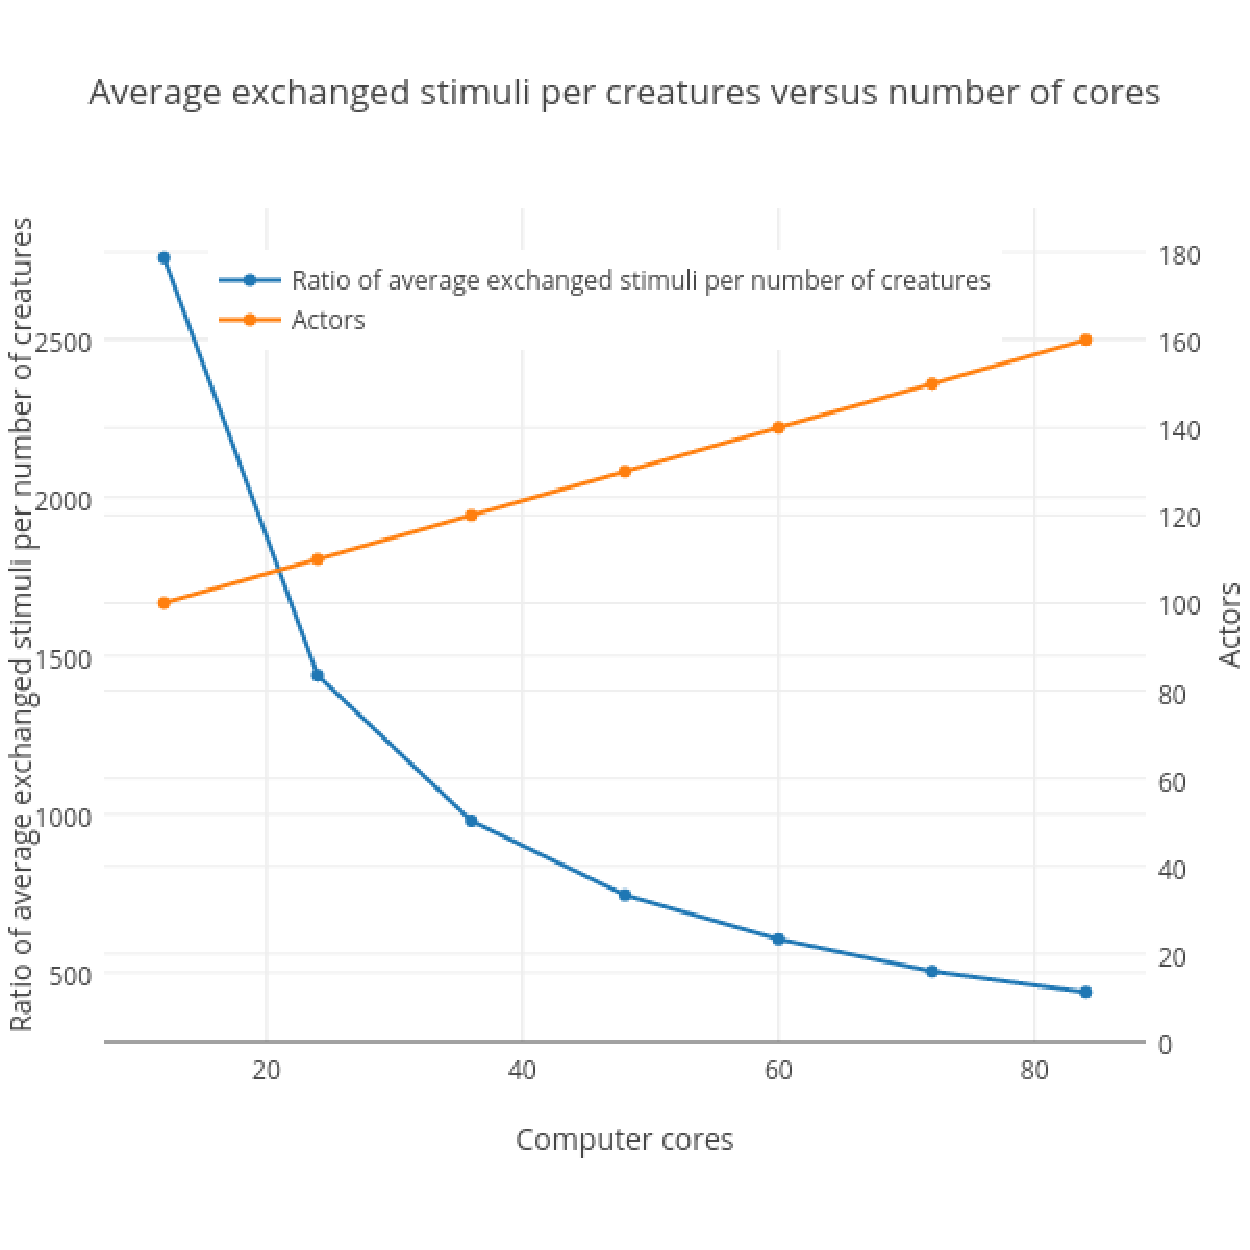
\includegraphics[scale=0.35]{images/ratioCreature}
	\caption{Average of exchanged stimuli over number of creatures versus number of computer cores. Each computer node possesses 12 cores.}
	\label{inferno}
\end{figure}

Fig. \ref{inferno} shows in left axis the ratio of average of exchanged stimuli over number of creature, as well as the total number of actors in right axis. By increasing both the number of computers and creatures, the ratio curve tends to a constant, which means that the number of creatures grows faster than the average exchanged stimuli. This is the expected behavior because the nutrient density in the world does not change and all the creatures operate in the same manner, thus exchanging approximately the same amount of stimuli.

%% talk about the increase in the upper bound of creatures per machine, as the new is twenty

\subsection{Model validity}
A experiment were designed aiming to compare the version using actor model and the former version, based on threads and shared memory, and verify the correctness of the first. It consists of a simple open-ended (the simulation finish when the creature dies) foraging simulation with one creature and ninety nutrients. It was repeated 50 times for both versions of architecture. As the system has a spacial dynamics. Fig. \ref{tracing} shows the superimposed path covered by 30 creatures in both implementations. It can be seen the creatures tend to cover all space. Simulations with more creatures shows an increased covered area and indicates that the system as a whole, seems to be ergodic \cite{Cornfeld2012}. It also show that the creatures are not skewed in just one direction.

\begin{figure*}[h]
	\centering
	\begin{subfigure}[t]{1\textwidth}
		\centering
		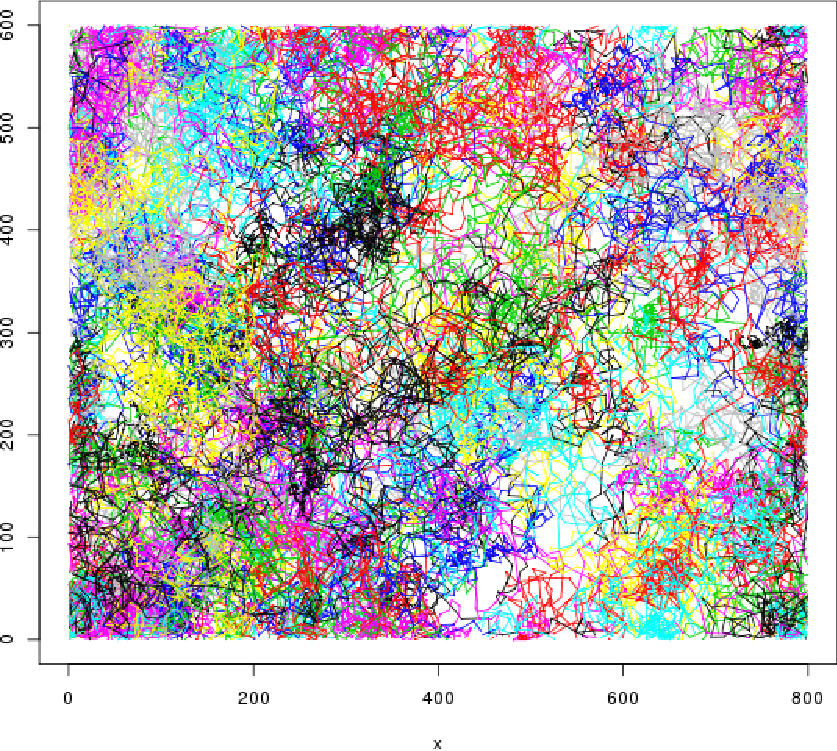
\includegraphics[height=8cm]{images/tracingAkka}
		\caption{implementation with actor model}
		\label{trace:akka}
	\end{subfigure}%
	\\
	\begin{subfigure}[t]{1\textwidth}
		\centering
		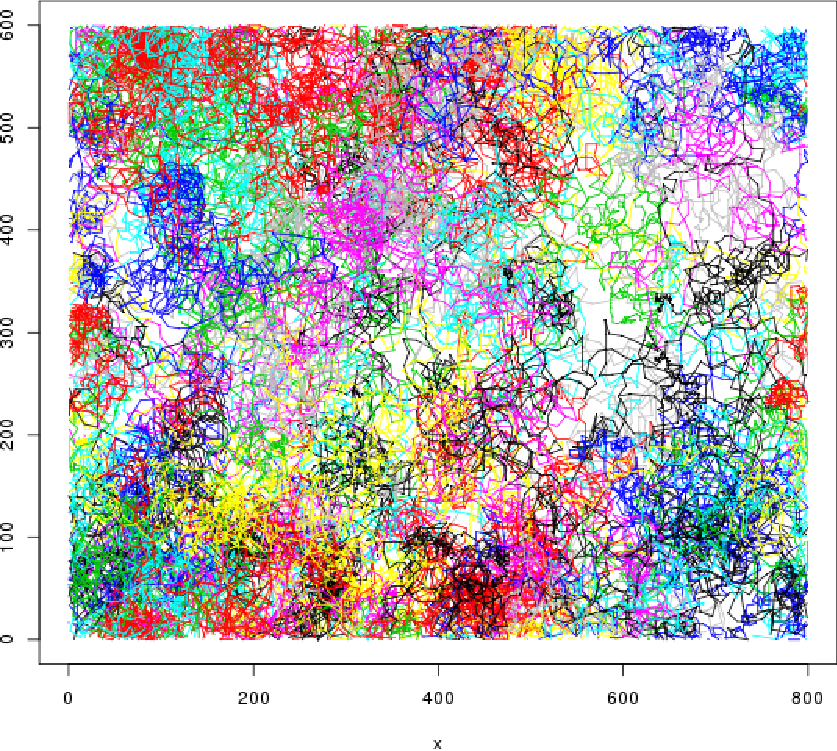
\includegraphics[height=8cm]{images/tracingNoAkka}
		\caption{implementation without actor model}
		\label{trace:noAkka}
	\end{subfigure}%
	~
	\caption{Two dimensional plot of superimposed world exploration by 30 independent creatures a) in an actor-based implementation b) in a classical implementation (using threads and shared memory) }
	\label{tracing}
\end{figure*}


Hunger deprivation is the difference between the metabolic consumption of a creature and it's energetic income from nutrients, measured in arbitrary units \cite{Campos}. The metabolism is constant, thus the hunger deprivation grows at constant rate. It reduces when the creature eats, with intensity equivalent to nutrient's energetic value. When the deprivation reaches 7, the creature dies. \autoref{deprivation} shows the hunger deprivation of a typical creature (\textit{i.e.}, a creature whose lifetime is close to the mean lifetime of all creatures) of both implementations. 

Behavioral efficiency is a function of the hunger deprivation that determines the speed and the opening of the creature's vision field, thus changing it ability to find food. It was modeled according to Yerkes-Dodson law \cite{Yerkes1908} and differs simple and complex tasks efficiency. A simple task is the one made by a creature when sensing only one nutrient while the complex task happens when there are more than one in the sensitive field. 

The \autoref{behavior} shows the temporal mean of behavioral efficiency for both implementations. The creature's behavior are similar in both versions, which means the creatures of the new implementation retained a coherent behavior. In \autoref{fig:behaviorWithAkka} there is a shrinkage on time axis, caused by changes made on the system to implement the actor model, which can be corrected by tunning the creature's metabolic rate. In either \autoref{fig:behaviorWithAkka} and \autoref{fig:behaviorWithout}, the majority of the creatures is dead from 0.15 hours on, and the results are no longer statistically valid, due to the sampling error.
 \newpage



\begin{figure*}[h]
	\centering
	\begin{subfigure}[t]{1\textwidth}
		\centering
		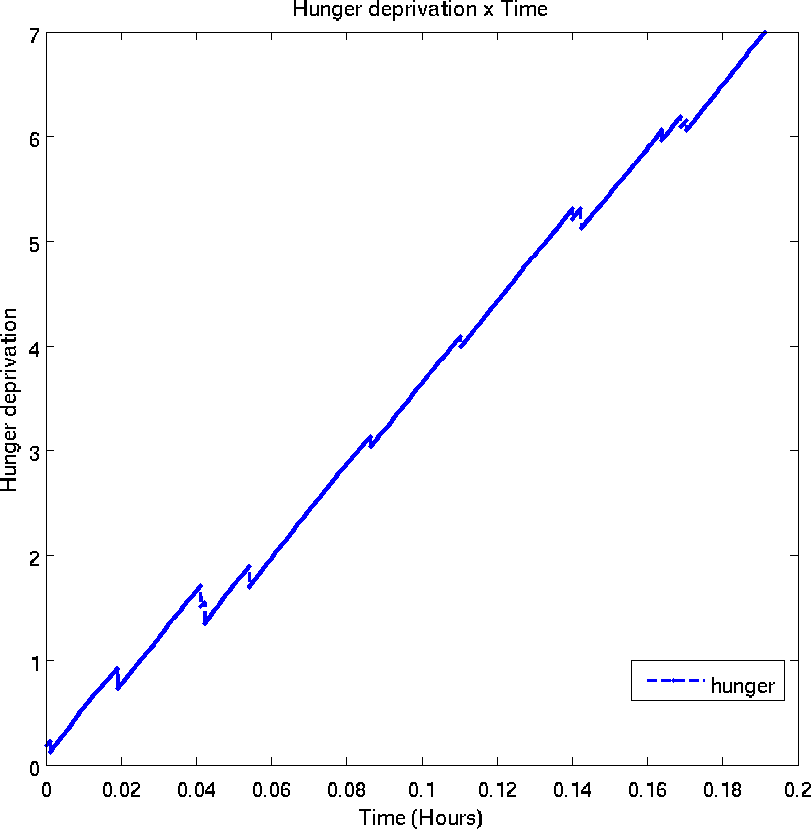
\includegraphics[height=8cm]{images/arousalAkka}
		\caption{implementation with actor model}
		\label{fig:arousalWithAkka}
	\end{subfigure}%
	\\
	\begin{subfigure}[t]{1\textwidth}
		\centering
		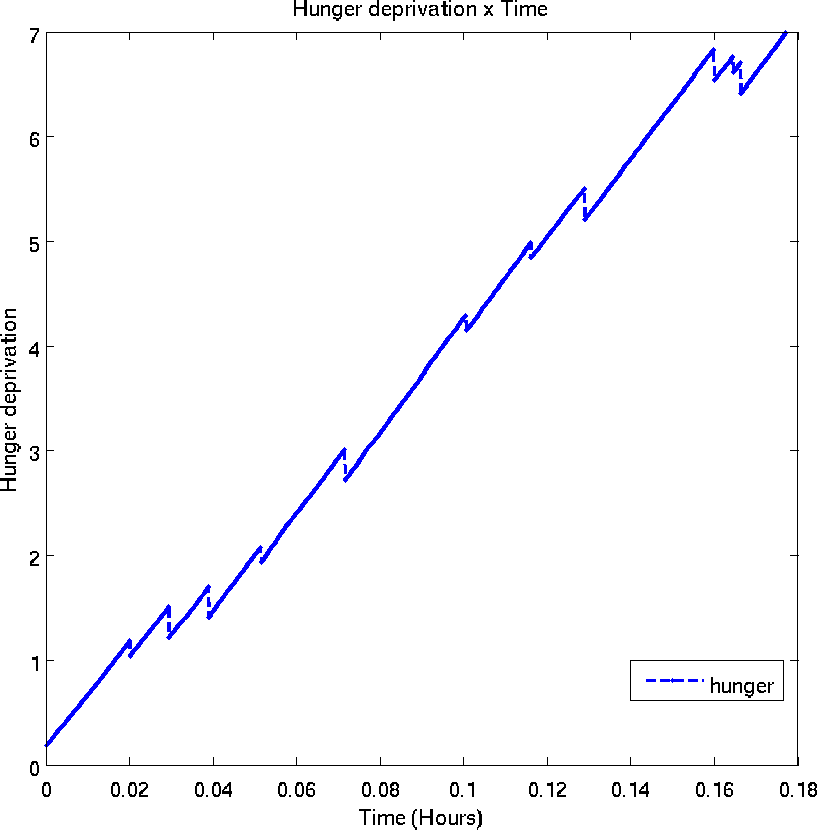
\includegraphics[height=8cm]{images/arousalNoAkka}
		\caption{implementation without actor model}
		\label{fig:arousalWithout}
	\end{subfigure}
	\caption{Hunger deprivation a typical creature of both implementations. }
	\label{deprivation}
\end{figure*}

\begin{figure*}[h]
	\centering
	\begin{subfigure}[t]{1\textwidth}
		\centering
		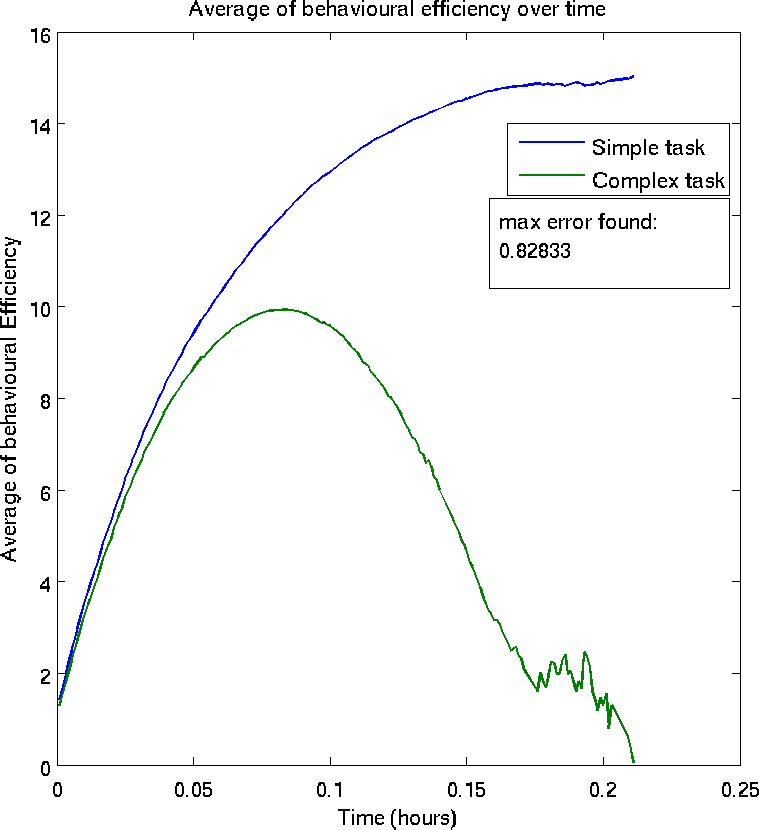
\includegraphics[height=8cm]{images/efficienceAkka}
		\caption{implementation with actor model}
		\label{fig:behaviorWithAkka}
	\end{subfigure}%
\\ 
	\begin{subfigure}[t]{1\textwidth}
		\centering
		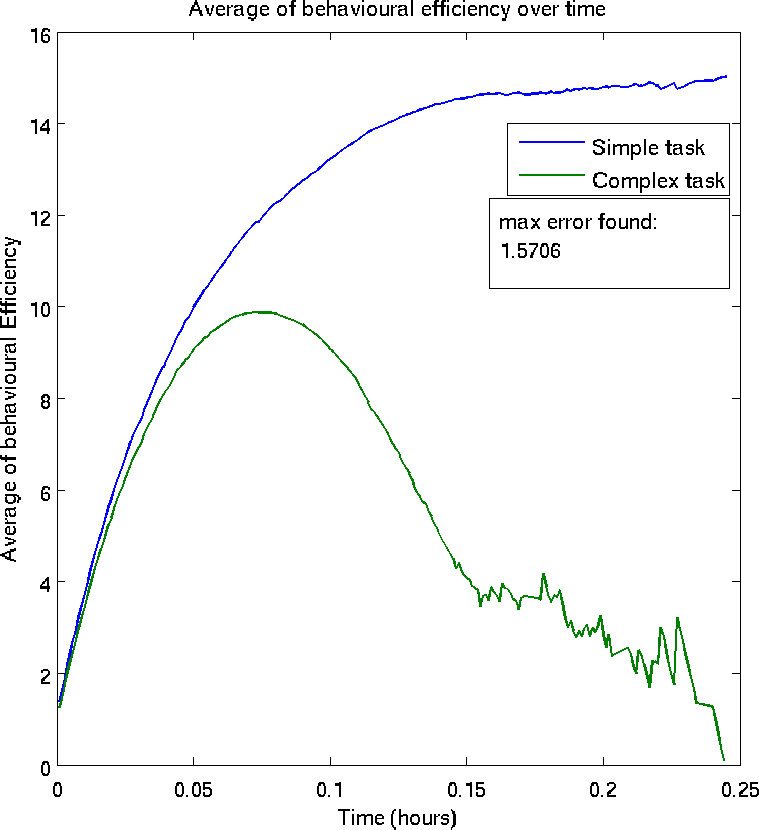
\includegraphics[height=8cm]{images/efficienceNoAkka}
		\caption{implementation without actor model}
		\label{fig:behaviorWithout}
	\end{subfigure}
	\caption{Behavioral efficiency of creatures in both implementations. }
	\label{behavior}
\end{figure*}

\newpage

\section{Conclusion}
\label{sec:conclusion}
The L2L architecture were used as a foraging simulator, and while there are many more simulators of this kind, L2L has a non-deterministic spatially-explicit and temporal dynamics. Also, the system seems to be ergodic, a point which needs further investigation. It was built having in mind the perspective of simulating population dynamics, however the scalability problems we face have made it infeasible. nonetheless, through using the actor model, we were able to scale out the architecture to multiple machines, clusterized or not, and reopen new research possibilities, including ecological simulations. A work in this direction is currently being done and will be published elsewhere. Finally, the toolkit we have adopted fits well enough our purposes as our system model is asynchronous and fault tolerant. Actor-based approach may not be appropriate to all MAS, mainly those not presenting these traits, albeit other nontraditional implementations of actor model may be useful in such scenarios.


\section*{Acknowledgment}

\noindent 
\includegraphics[width=0.6cm]{bandeira.png} This project has received funding from the European Union’s Horizon 2020 research and innovation programme under the Marie Skłodowska-Curie grant agreement No 754382. This research has also been partially supported by Comunidad de Madrid, PROMINT-CM project (grant ref: P2018/EMT-4366) and by the project PID2020-115454GB-C21 of the Spanish Ministry of Science and Innovation (MICINN). The authors thank UAH, UFRJ and CEFET-MG for the infrastructure, and Brazilian research agencies for partially support: CAPES (Finance Code 001), FAPERJ, and National Council for Scientific and Technological Development – CNPq. ``The content of this publication does not reflect the official opinion of the European Union. Responsibility for the information and views expressed herein lies entirely with the author(s).''


\FloatBarrier


%

%
% ---- Bibliography ----
%
% BibTeX users should specify bibliography style 'splncs04'.
% References will then be sorted and formatted in the correct style.
%
\bibliographystyle{splncs04}
\bibliography{references}
%

\end{document}
